\documentclass[]{article}
\usepackage[top=2.5cm, bottom=2.5cm, left=3cm, right=3cm]{geometry}
\usepackage{amsmath,amssymb,amsfonts,latexsym,textcomp} %paquetes matematicos
\usepackage{array,multirow,booktabs,tabulary} %tablas y arrays
\usepackage{graphicx}   
\usepackage{caption,float,subfigure} %float=figuras flotantes.
\usepackage{verbatim}  %texto raw 
\usepackage[ampersand]{easylist} %http://en.wikibooks.org/wiki/LaTeX/List_Structures#Easylist_package 
\usepackage{subfigure}
\usepackage{color}
\usepackage[usenames,dvipsnames,svgnames,table,x11names]{xcolor} 

%---- Usar otros fonts + símbolo \degree -----------------------------------
\newcommand*{\myfont}{\fontfamily{lmtt}\selectfont}
\DeclareTextFontCommand{\textmyfont}{\myfont}	
\usepackage{gensymb} 

%---- Code highlighting con Listings ---------------------------------------
\usepackage{listings}	
\definecolor{mygreen}{rgb}{0.5,0.6,0.5}
\definecolor{mygray}{rgb}{0.5,0.5,0.5}
\definecolor{mymauve}{rgb}{0.58,0,0.82}
\definecolor{mygray2}{rgb}{0.9764, 0.9764, 0.9762}
%---- Config listings ------------------------------------------------------
\lstset{ %
	backgroundcolor=\color{mygray2},	% background color
	basicstyle=\footnotesize\ttfamily,	% tamaño de las letras y tipo de letra
	breaklines=true,	% corte de linea (line breaking)solo en espacio blanco
	captionpos=t,		% posicion del caption b,t,n (top,bottom,none)
	commentstyle=\color{ForestGreen},	% estilo del comentario
	%escapeinside={\%*}{*},	% si se desea agregar codigo Latex dentro el codigo debe ser %*codigo latex*
	frame=single,	% agrega marco al codigo
	frameround=tttt,	% redondear el marco
	keepspaces=true,	% mantiene los espacios en el texto, util para mantener la indentacion del codigo (uso posible en columns=flexible)
	keywordstyle=\color{blue},	% estilo de los keywords
	stringstyle=\color{mymauve},	% estilo del string
	numbers=left,	% donde poner los numeros de linea, (none, left, right)
	numbersep=5pt,	% cuan lejos los numeros de linea estan del codigo
	xleftmargin=0pt,	% margen izquierdo
	showspaces=false,	% muestra espacios de codigo en todas partes usando el caracter barra baja "_", sobreescribe el comando 'showstringspaces'
	showstringspaces=false,	% muestra espacios solo en los strings
	tabsize=2,	% tabulacion por defecto =2
	title=\lstname	% muestra el nombre de lo archivos incluidos con \lstinputlisting; tambien se puede tratar con caption en vez de title
}	
%---- Config personalizada del caption -------------------------------------
\DeclareCaptionFont{white}{ \color{white} }
\DeclareCaptionFormat{listing}{
	\colorbox[cmyk]{0.43, 0.35, 0.35, 0.01 }{
		\parbox{0.96\linewidth}{\hspace{15pt}#1#2#3}
	}
}
\captionsetup[lstlisting]{ format=listing, 
	labelfont=white, 
	textfont=white, 
	singlelinecheck=false, 
	margin=0pt, 
	font={bf,footnotesize} }
%---- Caracteres especiales ------------------------------------------------	
% Por defecto, listings no soporta inputec para mostrar los acentos y caracteres especiales.
% para manejar utf8 se debe enlistar los caracteres segun:
\lstset{literate=
	{á}{{\'a}}1 {é}{{\'e}}1 {í}{{\'i}}1 {ó}{{\'o}}1 {ú}{{\'u}}1
	{Á}{{\'A}}1 {É}{{\'E}}1 {Í}{{\'I}}1 {Ó}{{\'O}}1 {Ú}{{\'U}}1
	{à}{{\`a}}1 {è}{{\`e}}1 {ì}{{\`i}}1 {ò}{{\`o}}1 {ù}{{\`u}}1
	{À}{{\`A}}1 {È}{{\'E}}1 {Ì}{{\`I}}1 {Ò}{{\`O}}1 {Ù}{{\`U}}1
	{ä}{{\"a}}1 {ë}{{\"e}}1 {ï}{{\"i}}1 {ö}{{\"o}}1 {ü}{{\"u}}1
	{Ä}{{\"A}}1 {Ë}{{\"E}}1 {Ï}{{\"I}}1 {Ö}{{\"O}}1 {Ü}{{\"U}}1
	{â}{{\^a}}1 {ê}{{\^e}}1 {î}{{\^i}}1 {ô}{{\^o}}1 {û}{{\^u}}1
	{Â}{{\^A}}1 {Ê}{{\^E}}1 {Î}{{\^I}}1 {Ô}{{\^O}}1 {Û}{{\^U}}1
	{œ}{{\oe}}1 {Œ}{{\OE}}1 {æ}{{\ae}}1 {Æ}{{\AE}}1 {ß}{{\ss}}1
	{ç}{{\c c}}1 {Ç}{{\c C}}1 {ø}{{\o}}1 {å}{{\r a}}1 {Å}{{\r A}}1
	{ñ}{{\~n}}1 {£}{{\pounds}}1 {°}{{\degree}}1
}		
%---- Macro de inclusión de documentos con listings ------------------------
% [2]=numero de argumentos, #1=argumento 1, #2=argumento 2
\newcommand{\includecode}[2]{\lstinputlisting[language=#1, caption=#2, label=#2]{#2}}			

%=============================================================================================
%opening
\title{EE4323 Industrial Control Systems\\ 
	Homework Assignment 2}
\author{Paulo R. Loma Marconi}

\begin{document}
\maketitle

\section{Raw model}

\begin{align}
e_{in}(t) &= R_A\ i_A + L_A\ \dot{i_A}+\alpha\ \omega_1 \\
J_1\ \dot{\omega_1} + B_1\ \omega_1 &= \alpha\ i_A + R_1\ f_c \\
J_2\ \dot{\omega_2} + B_2\ \omega_2 + B_{2C}\ sign(\omega_2) &= -\tau_{LE}-R_2\ f_c \\
C_{TM}\ \dot{\theta_M} + (\theta_M - \theta_A)/R_{TM} &= i^2_A\ R_A
\end{align}

Which delivers in sate-vector differential equations  
$x = [ i_A\ \omega_2\ \theta_M ]^T $ and input $u = [ e_{in}\ \tau_{LE}\ \theta_A ]^T$.

\begin{align}
\dot{i_A} &= -a\ i_A - b\ \omega_2 + e_{in}/L_A \\
\dot{\omega}_2 &= c\ i_A - d\ \omega_2 - e\ sign(\omega_2) - \tau_{LE}/J_{eq}\\
\dot{\theta}_M &= f\ i^2_A - g\ \theta_M + g\ \theta_A
\end{align}

Where,
\begin{align*}
&J_{eq}=J_2+N^2\ J_1;\quad B_{eq}=B_2+N^2\ B_1\\
&a=R_A/L_A;\quad b=\alpha\ N/L_A\\
&c=N\ \alpha/J_{eq};\quad d=B_{eq}/J_{eq};\quad e=B_{2C}/J_{eq}\\
&f=R_A/C_{TM};\quad g=1/(C_{TM} R_{TM})
\end{align*}

\section{Code and simulation}
In \verb|asst02.m| it can be seen the input and the state-vector differential equations, and \verb|run asst02.m| is the code for the simulation of  Fig.\ref{fig:point2}.

\begin{lstlisting}[language=matlab, caption={asst02.m}, label={asst02}]
function xdot = asst02_2017(t,x)
global E_0 Tau_0 T_Amb B_2C %%% make these settable from a script
% motor parameters, Nachtigal, Table 16.5 p. 663
J_1 = 0.0035; % in*oz*s^2/rad
B_1 = 0.064; % in*oz*s/rad
% electrical/mechanical relations
K_E = 0.1785; % back emf coefficient, e_m = K_E*omega_m (K_E=alpha for omega)
K_T = 141.6*K_E; % torque coeffic.; in English units K_T is not = K_E! (K_T=alpha for iA) 
R_A = 8.4; % Ohms
L_A = 0.0084; % H
% gear-train and load parameters
J_2 = 0.035; % in*oz*s^2/rad % 10x motor J
B_2 = 2.64; % in*oz*s/rad (viscous)
N = 8; % motor/load gear ratio; omega_1 = N omega_2
% Thermal model parameters
R_TM = 2.2; % Kelvin/Watt
C_TM = 9/R_TM; % Watt-sec/Kelvin (-> 9 sec time constant - fast!)

Jeq=J_2+N*2*J_1;
Beq=B_2+N^2*B_1;
a=R_A/L_A;
b=K_E*N/L_A;
c=N*K_T/Jeq;
d=Beq/Jeq;
e=B_2C/Jeq;
f=R_A/C_TM;
g=1/(C_TM*R_TM);

if t < 0.05,
	e_i = 0;
else  
	e_i = E_0;  
	%e_i = E_0*sin(2*pi*5*(t - 0.05)); 
end
if t < 0.5
	Tau_L = 0;
else
	Tau_L = Tau_0;
end

xdot(1) = -a*x(1)-b*x(2)+e_i/L_A;
xdot(2) = c*x(1)-d*x(2)-e*sign(x(2))-Tau_L/Jeq;
xdot(3) = f*x(1)^2-g*x(3)+g*T_Amb;
\end{lstlisting}

\begin{lstlisting}[language=matlab, caption={run asst02.m}, label={runasst02}]
clear; close all; clc;
global E_0 Tau_0 T_Amb B_2C ;

E_0 = 120; Tau_0 = 80; T_Amb = 18; B_2C = 80;
t0 = 0; tfinal = 1.2; stp = 0.0001;
x0 = [ 0;0;0 ]; %initial conditions

timer = clock;
[t1,x1] = ode45m('asst02_2017',t0,tfinal,x0,stp);
Tsim1 = etime(clock,timer), % integration time 
Len1 = length(t1), % number of time-steps

figure

subplot(3,1,1)       
plot(t1,x1(:,1));
title('Motor+Load+thermal model simulation, B_{2C}=80')
xlabel('Time, t (sec)')
ylabel('i_A (amperes)')
text(0.2,1,['E_0 =',num2str(E_0,3)]);

subplot(3,1,2)       
plot(t1,x1(:,2));
title('Motor+Load+thermal model simulation, B_{2C}=80')
xlabel('Time, t (sec)')
ylabel('\omega_2 , Motor angular velocity (rad/sec)')
text(0.2,24,['B_{2C} =',num2str(B_2C,3),'\tau_0 =',num2str(Tau_0,3)]);

subplot(3,1,3)      
plot(t1,x1(:,3));
title('Motor+Load+thermal model simulation, B_{2C}=80')
xlabel('Time, t (sec)')
ylabel('\theta_M (deg)')
text(0.2,5,['\Theta_A=',num2str(T_Amb,3) ' deg']);

\end{lstlisting}

\begin{figure}
	\centering
	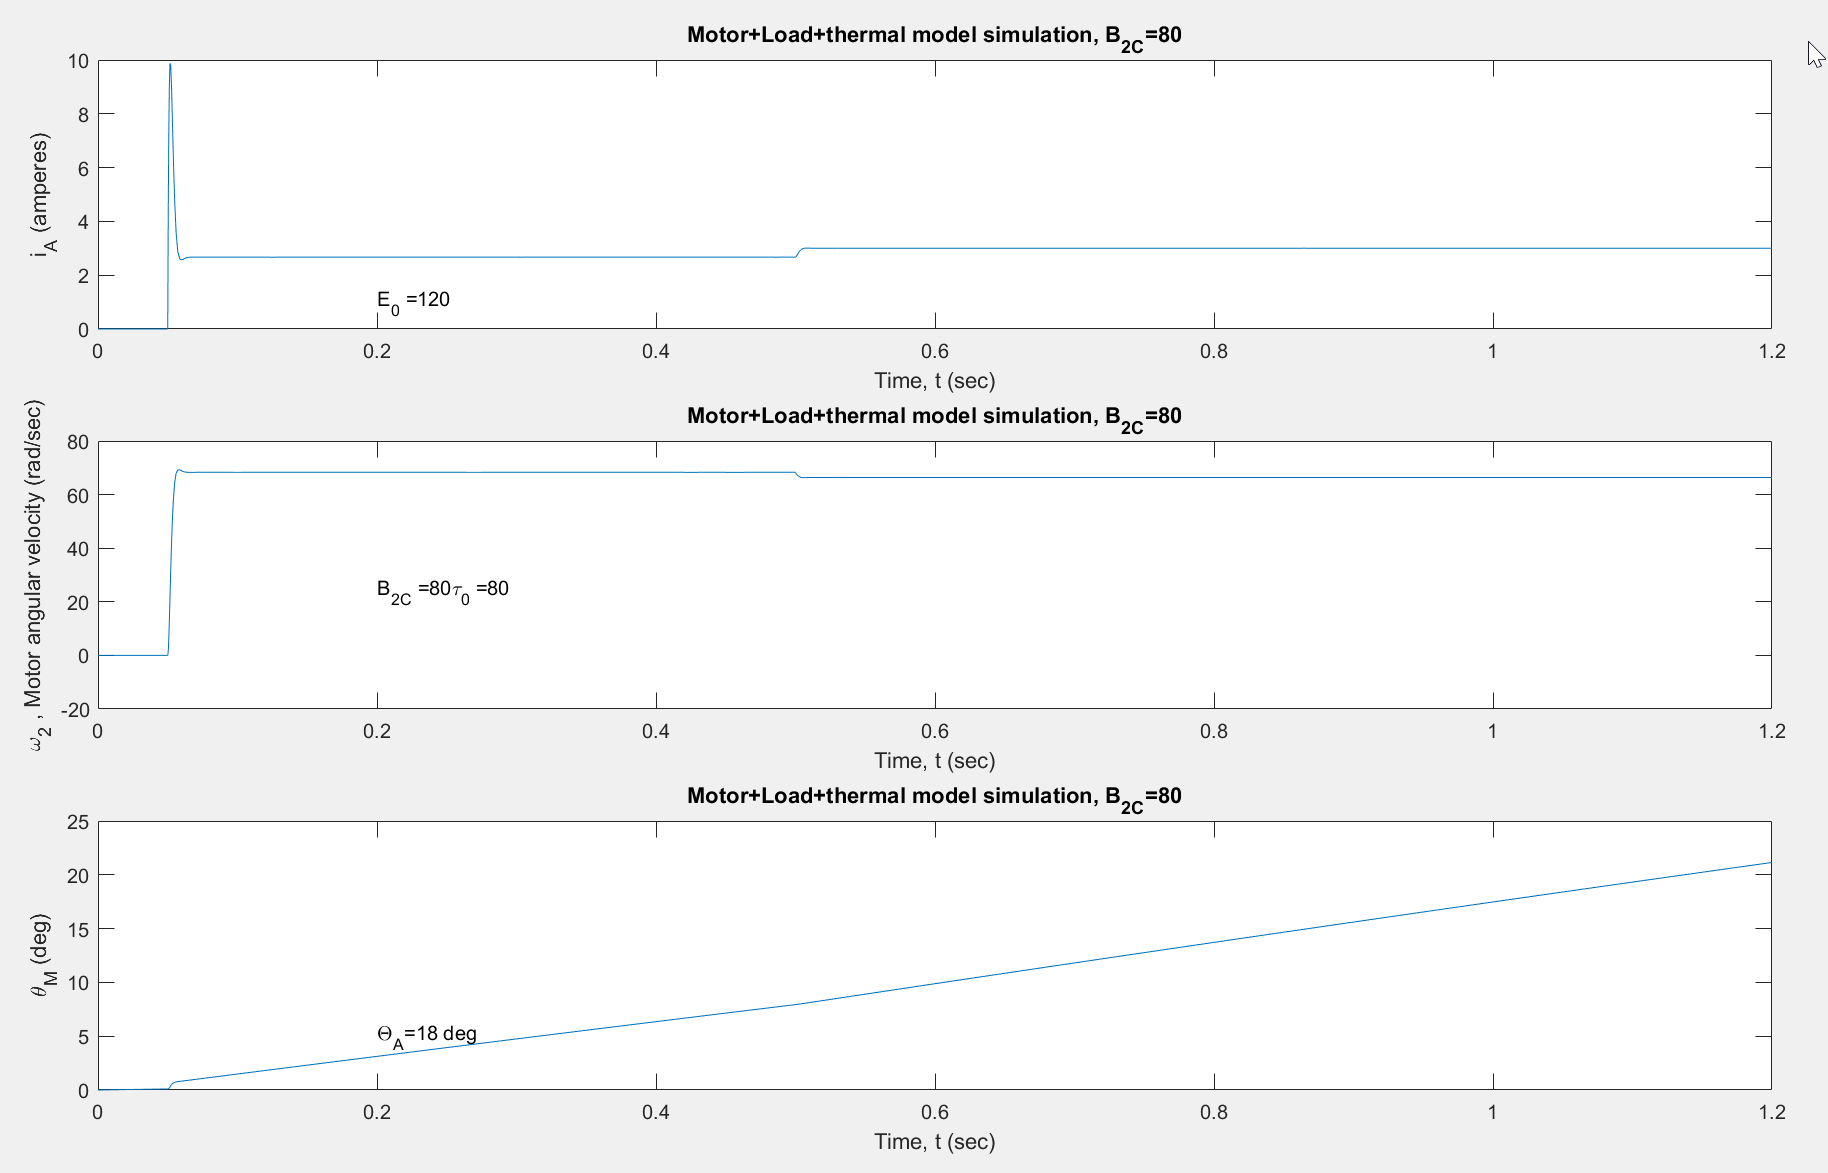
\includegraphics[width=1\linewidth]{point2}
	\caption{Simulation for Q. 2}
	\label{fig:point2}
\end{figure}

The high current peak in before 0.1 sec is because of the inertia that the motor has to overcome, after it breaks the inertia the amount of current drops down to a constant value. In 0.5 sec the $\tau_{LE}$ is applied and we can see an increment of the current and a decrease of the angular velocity.

\section{Ode45 vs eufix1}
In Fig.\ref{fig:ode45_vs_eufix1} can be seen that the \textbf{maximum peak current} for ode45 and eufix1 at two different integration steps, \textbf{1e-4} and \textbf{1e-3}.

\begin{figure}
	\centering
	\subfigure[ode45 with step=1e-4]{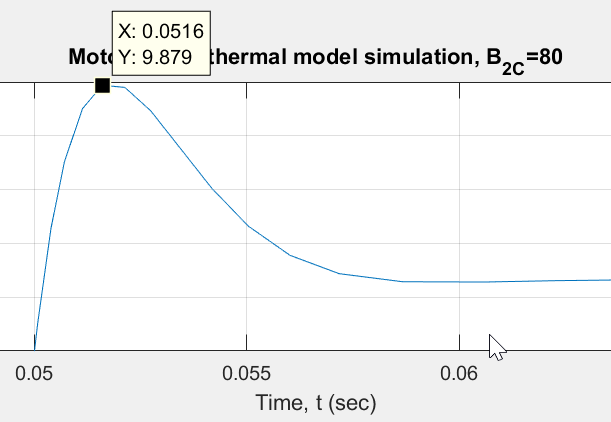
\includegraphics[width=0.45\linewidth]{ode45_1e-4.png}}
	\subfigure[eufix1 with step=1e-4]{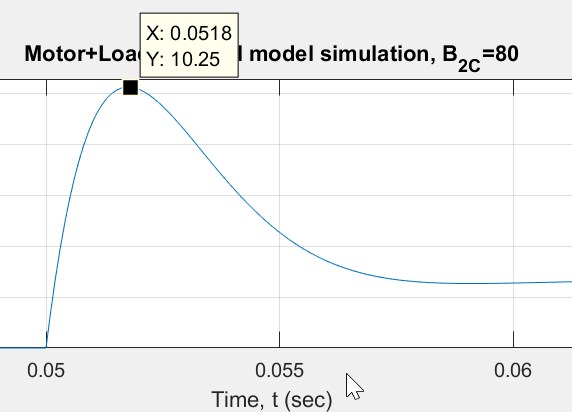
\includegraphics[width=0.43\linewidth]{eufix1_1e-4.png}}
	\subfigure[ode45 with step=1e-3]{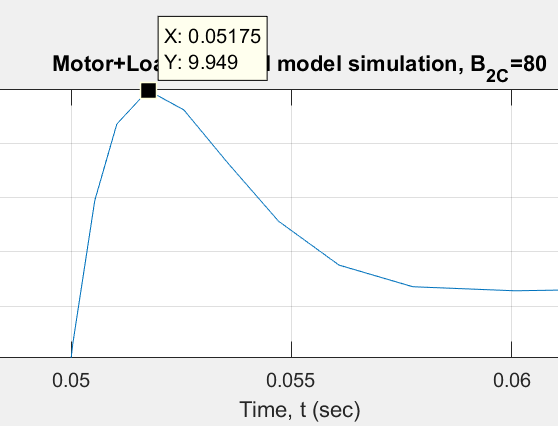
\includegraphics[width=0.43\linewidth]{ode45_1e-3.png}}
	\subfigure[eufix1 with step=1e-3]{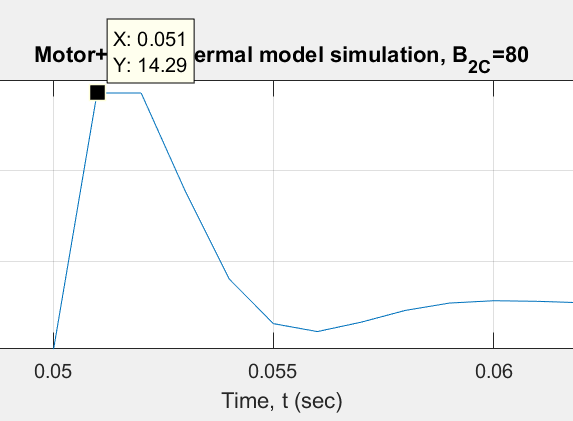
\includegraphics[width=0.45\linewidth]{eufix1_1e-3.png}}
	\caption{Maximum peak current with \textbf{ode45 vs eufix1}}
	\label{fig:ode45_vs_eufix1}
\end{figure}

There is little difference between ode45 and eufix at step=1e-4 but when we change to step=1e-3 there a big difference, about 70\% more.

The number of time steps is given by the instruction \verb|Len1 = length(t1),| which delivers two results, \verb|Len1 = 663| for \verb|ode45| and \verb|Len1 = 1202| for \verb|eufix1|.

\section{Will the motor melt?}
Fig.\ref{fig:melt} shows that the maximum temperature is 182.4\degree C at time 40 sec, which means that the heating it's not enough to melt the metal of the motor that could be around 700\degree C if it's made of Aluminum or 419\degree C if it has Zinc. 

\begin{figure}
	\centering
	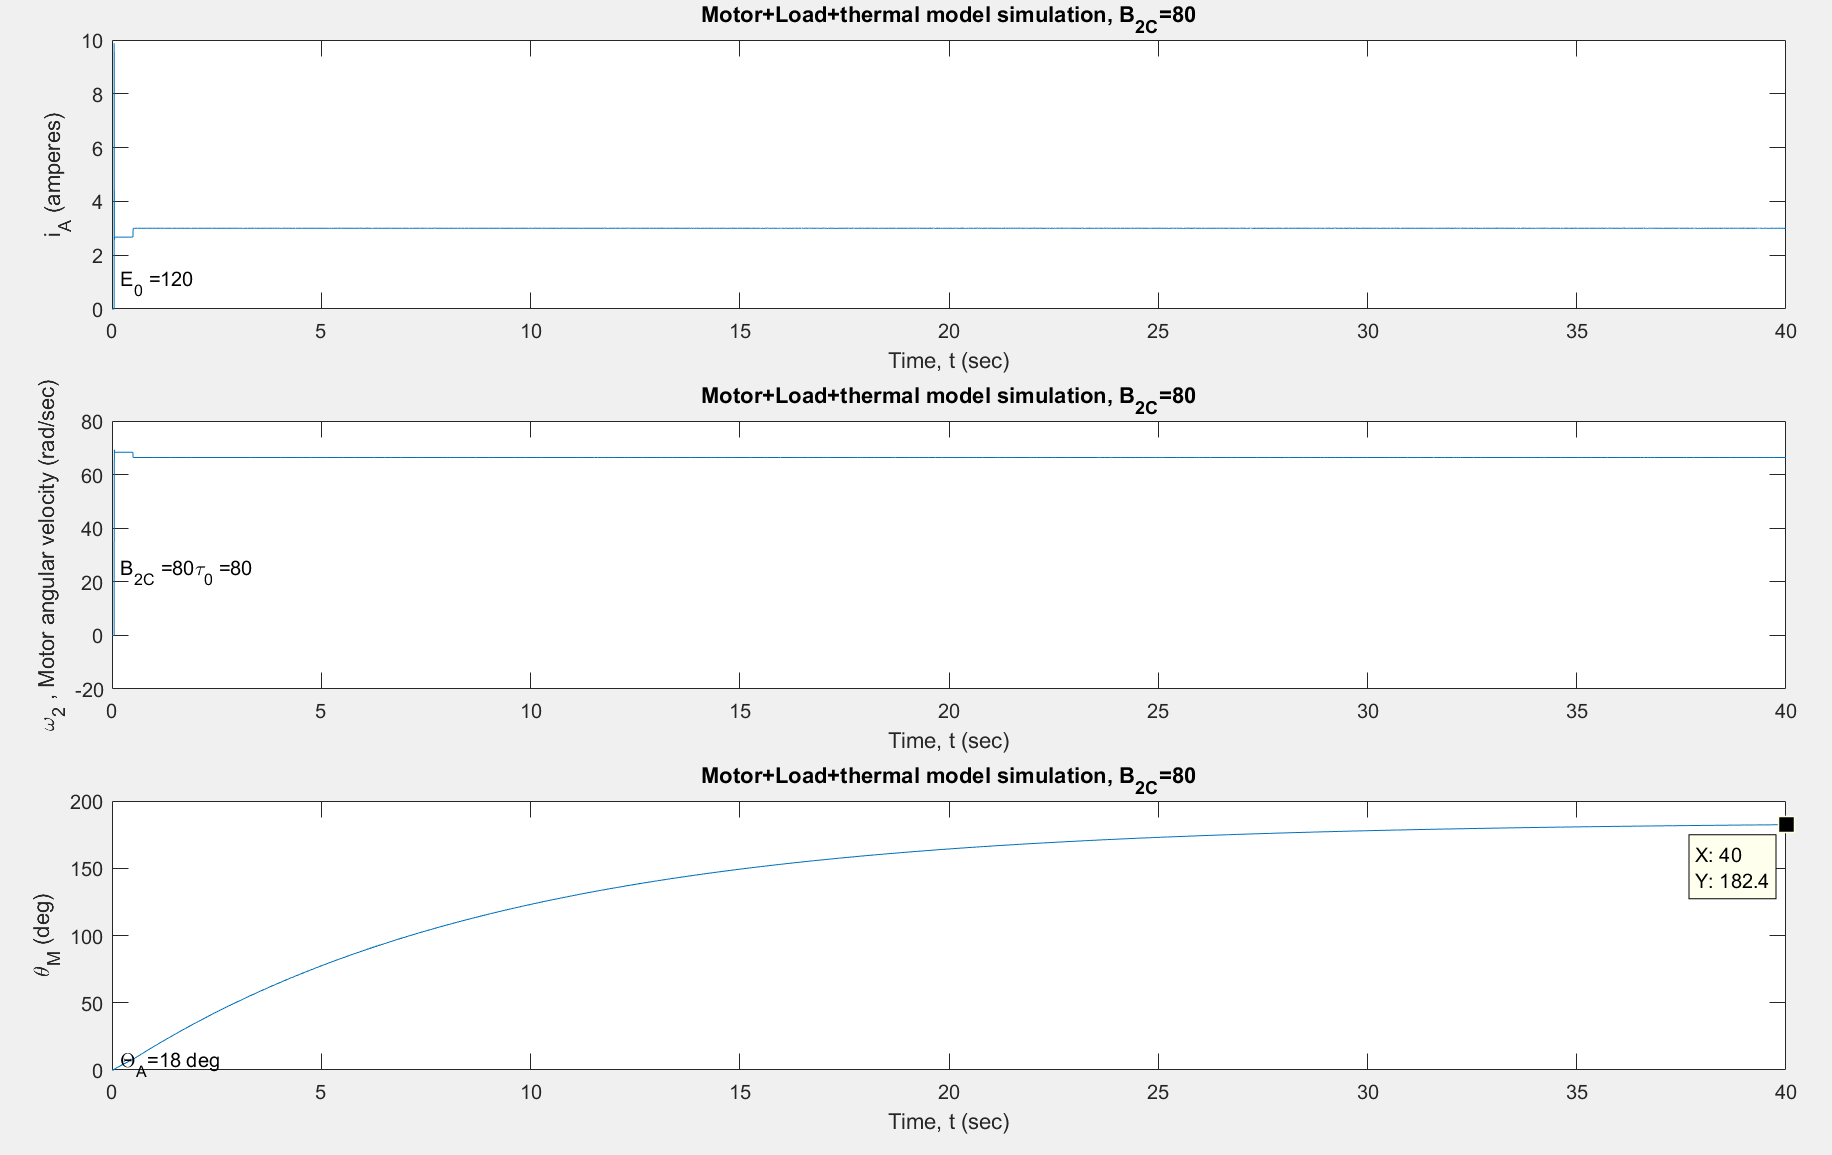
\includegraphics[width=1\linewidth]{melt}
	\caption{Ode45 simulation with t = 40sec}
	\label{fig:melt}
\end{figure}

\section{Motor is continually reversing at 5Hz}
Fig.\ref{fig:reversing} shows the result of 5 cycles with an 5Hz of input; \verb|e_i = E_0*sin(2*pi*5*(t - 0.05))|, and with a 6315 time steps for \verb|ode45| and 10002 time steps for \verb|eufix1|.
\begin{figure}
	\centering
	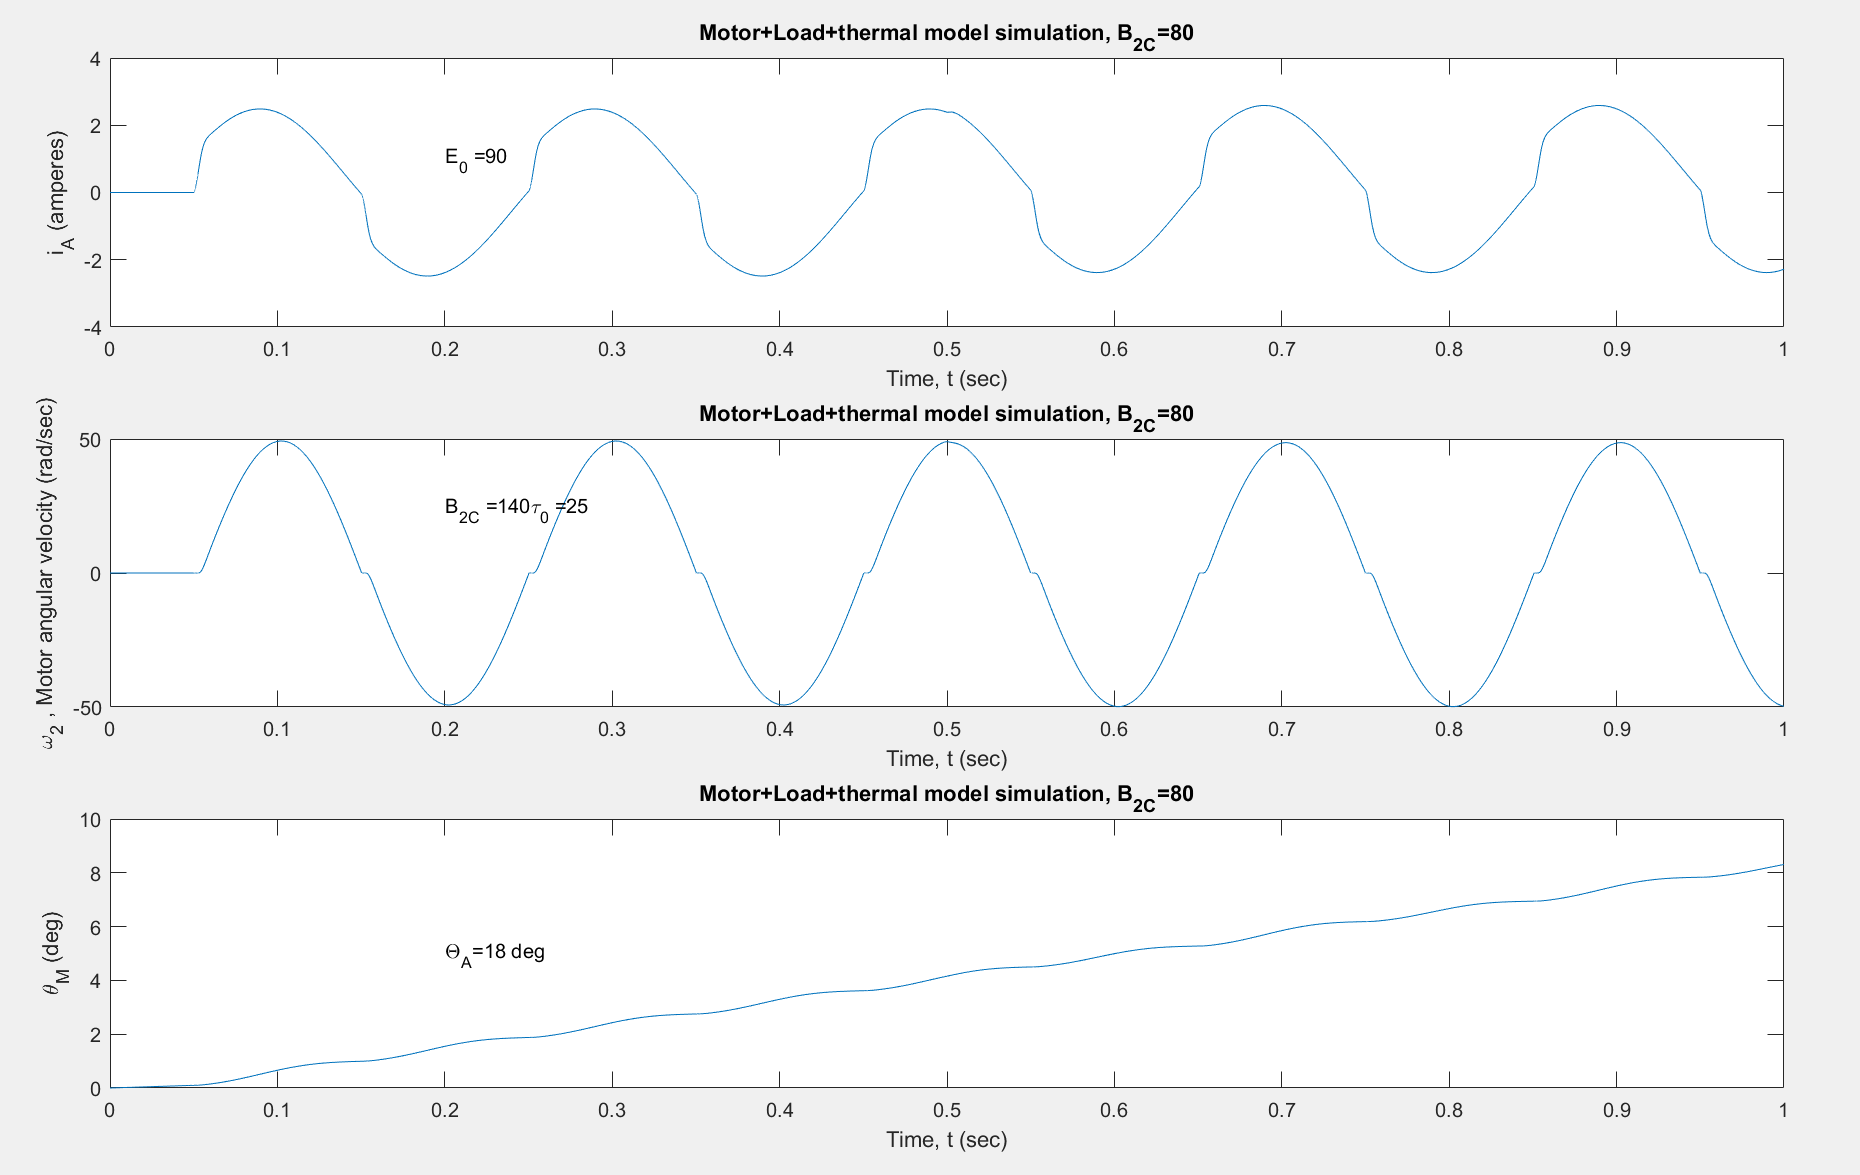
\includegraphics[width=1\linewidth]{reversing}
	\caption{Motor at 5Hz}
	\label{fig:reversing}
\end{figure}




\end{document}
